\section{Analoog}
\subsection{De opdracht}
\begin{minipage}{0.45\textwidth}
	Maak een derde orde 0.5dB ripple chebyshev lowpass filter met een $F_C$ van 70Hz. In de doorlaat band 
	moet er met 10dB worden versterkt. Uit de tabel zijn de volgende gegevens te halen.
\end{minipage}
\hfill
\begin{minipage}{0.45\textwidth}
	\begin{itemize}
		\item In doorlaat +10dB versterking
		\item $\omega_{0_1}=1.0688$ 
		\item $\omega_{0_2}=0.6265$
		\item $\alpha = 0.5861$
		\item $Q=\frac{1}{\alpha}=1.7061$
	\end{itemize} % Gegevens komen uit tabel 8.30 van het boek linear circuit design
\end{minipage}

\subsection{Overdracht bepalen}
\begin{minipage}{0.40\textwidth}
	Door de waardes uit de tabel in te vullen in de standaard formule (zie formule \ref{eq:hs})
	komt daar formule \ref{eq:hsNum} uit.

	\noindent
	H(s) kan worden opgesplitst in een tweede orde deel en een eerste orde deel zie formule \ref{eq:hsSplit}.
	Het opsplitsen van $H(s)$ in $H(s)_1$ en $H(s)_2$ is noodzakelijk voor het goed ontwerpen van het analoge 
	filter.

	\noindent
	Het tweede orde deel heeft de overdracht die te zien is in formule \ref{eq:hs1} en de overdracht van
	het eerste orde	deel is te zien in formule \ref{eq:hs2}
\end{minipage}
\hfill
\begin{minipage}{0.60\textwidth}
	\begin{align}
		H(s)&=\frac{(\omega_{0_1}\cdot\omega_c)^2\cdot\omega_c\cdot\omega_{0_2}}{(s^2+ \alpha \cdot \omega_{0_1} \cdot \omega_c \cdot s + (\omega_{0_1}\cdot\omega_c)^2)\cdot (s + \omega_c \cdot \omega_{0_2})} \label{eq:hs} \\
		H(s)&=\frac{220\, 156.6429\,\cdot\, 275.0335}{(s^2+274.9999\cdot s+220\, 156.6429)(s+275.0335)} \label{eq:hsNum}\\
		H(s)&= H(s)_1 \cdot H(s)_2 \label{eq:hsSplit} \\ 
		H(s)&_1=\frac{(\omega_{0_1}\cdot\omega_c)^2}{s^2+ \alpha \cdot \omega_{0_1} \cdot \omega_c \cdot s + (\omega_{0_1}\cdot\omega_c)^2} \label{eq:hs1} \\ 
		H(s)&_2=\frac{\omega_c\cdot\omega_{0_2}}{s + \omega_c \cdot \omega_{0_2}} \label{eq:hs2} \\ 
	\end{align}
\end{minipage}
 
%$H(s)_1=\frac{220\, 156.6429}{s^2+274.9999s+220\, 156.6429}$
%$H(s)_2=\frac{275.0335}{s+275.0335}$

\subsection{Tweede orde/Sallen-key}
\begin{wrapfigure}[6]{l}{0.25 \textwidth}
	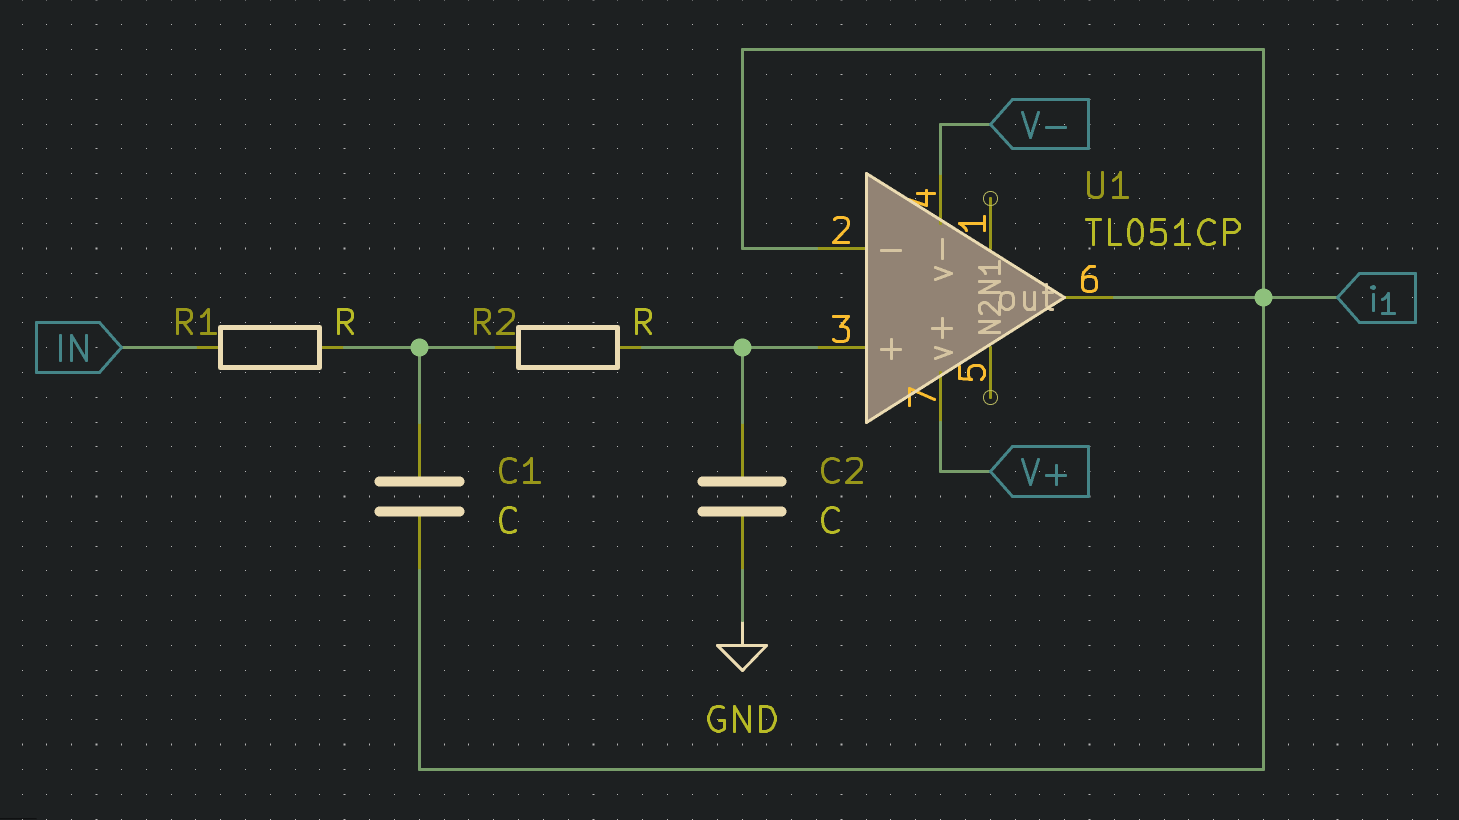
\includegraphics[width=0.9\linewidth]{schematic/sallenkay.png}
	\caption{Sallen-key}
	\label{fig:sallenKey}
\end{wrapfigure}

\vphantom{-}\\
\begin{minipage}{0.37\textwidth}
	Het tweede orde deel van het derde orde filter wordt via de Sallen-key topologie gerealiseerd. In afbeelding \ref{fig:sallenKey} is te zien 
	hoe een laag doorlaat sallen-key filter er uit ziet.
\end{minipage}
\hfill
\begin{minipage}{0.37\textwidth}
	\begin{equation} \label{eq:c1}
		C_1=\frac{2Q}{\omega_c\omega_{0_1}R}
	\end{equation}
	\begin{equation} \label{eq:c2}
		C_2=\frac{1}{2Q\omega_c\omega_{0_1}R}
	\end{equation}
\end{minipage}
\vphantom{-}\\

\noindent
Als $R_1 = R_2$ kan $C_1$ berekend worden met formule \ref{eq:c1} en $C_2$ met formule \ref{eq:c2}.
Voor dit filter is gekozen om voor R $10k\Omega$ te kiezen. Waardoor $C_1=727nF$.

\noindent
727nF is alleen niet een waarde waarin condensatoren worden gemaakt. Door $C_1$ te veranderen naar 750nF 
kan er wel een condensator worden gekocht met de juiste waarde. 

\noindent
Door $C_2$ met formule \ref{eq:c2} uit te rekenen komt $C_2$ uit op een waarde van 62nF, deze waarde is wel direct 
te koop. 

\noindent
Beide waardes zitten alleen niet in de E6/12 reeks en zijn dus aanzienlijk duurder, 
hier gaat een afweging meespelen tussen de prijs van componenten en de kwaliteit van het filter.

\subsection{Eerste orde}
\begin{wrapfigure}[5]{l}{0.25\textwidth}
	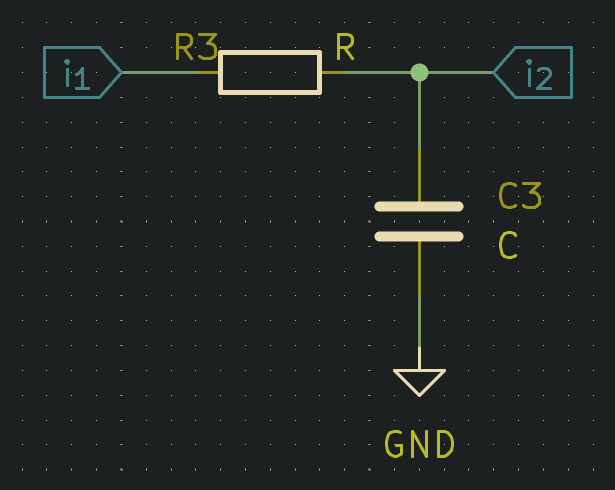
\includegraphics[width=0.9\linewidth]{schematic/rc.png}
	\caption{Eerste orde lp filter}
	\label{fig:lp}
\end{wrapfigure}
\vphantom{-}\\
Een passief eerste orde laag doorlaat filter staat in figuur \ref{fig:lp}. Met formule \ref{eq:rc} is het mogelijk om de verschillende component waardes uit te rekenen 
voor het filter. Wij hebben $C_3=100nF$ gekozen waaruit formule \ref{eq:rcValR} volgt dat 
$R_3=5787\Omega$ dit moet worden afgerond op $5.6k\Omega$ omdat er geen weerstanden beschikbaar zijn met een waarde van $5787\Omega$.

\begin{flushright}
	\begin{minipage}{0.37\textwidth}
		\begin{equation} \label{eq:rc}
			\omega_c*\omega_{0_2}=\frac{1}{R_3C_3}
		\end{equation}
	\end{minipage}
	\begin{minipage}{0.37\textwidth}
		\begin{equation} \label{eq:rcValR}
			R_3=\frac{1}{\omega_c*\omega_{0_2}C_3}
		\end{equation}
	\end{minipage}
\end{flushright}
\newpage
\subsection{LTspice}

\subsection{Metingen}
